\chapter{Determination of Rare Earth Elements in Hypersaline Solutions Using Low-Volume, Liquid-Liquid Extraction}
\chaptermark{LLE method for brines}

This chapter is adapted from a publication by the same name, co-authored by David A. Dzombak and Athanasios K. Karamalidis.
This paper is citable as: 

Noack, C. W.; Dzombak, D. A.; Karamalidis, A. K., Determination of Rare Earth Elements in Hypersaline Solutions Using Low-Volume, Liquid-Liquid Extraction. \textit{Environ. Sci. Technol.} \textbf{2015}, \textit{Article ASAP}, DOI: 10.1021/acs.est.5b00151

My contributions to this work were the experimental design; execution of experiments including ICP-MS analysis; data analysis and visualization; interpretation of results; and drafting of the manuscript.

\clearpage

\section*{Abstract}
Complex, hypersaline brines --- including those co-produced with oil and gas, rejected from desalination technologies, or used as working fluids for geothermal electricity generation --- could contain critical materials such as the rare earth elements (REE) in valuable concentrations.
Accurate quantitation of these analytes in complex, aqueous matrices is necessary for evaluation and implementation of systems aimed at recovering those critical materials.
However, most analytical methods for measuring trace metals have not been validated for highly saline and/or chemically complex brines.
Here we modified and optimized previously published liquid-liquid extraction (LLE) techniques [Shabani et al., \textit{Anal. Chem.} 1990, 62 (24) 2709-2714; Lawrence and Kamber, \textit{Geostand. Geoanal. Res.} 2007, 31 (2) 95-103], using bis(2-ethylhexyl) phosphate as the extractant in a heptane diluent, and studied its efficacy for REE recovery as a function of three primary variables: background salinity (as NaCl), concentration of a competing species (here Fe), and concentration of dissolved organic carbon (DOC).
Results showed that the modified LLE was robust to a range of salinity, Fe, and DOC concentrations studied as well as constant, elevated Ba concentrations.
With proper characterization of the natural samples of interest, this method could be deployed for accurate analysis of REE in small volumes of hyper-saline and chemically complex brines.

\section{Introduction}

The rare earth elements (REE) are among the most frequently cited critical materials for clean energy and high-tech manufacturing.1, 2 
The unique and varied properties of REE have led to their application in more consumer products than nearly any other element group.3
REE are mostly obtained from mining and processing of REE-enriched ores.2
While economically preferred, mining is laborious with a significant environmental burden, and inexpensive alternative sources of critical materials are sought after resources.

Aqueous byproduct or waste streams, both natural and industrial, are potential sources of the REE and other critical materials.
With increasing global interest in geothermal energy,4
development of unconventional oil and gas resources (e.g. hydraulic fracturing of organic rich shales),5
and desalination technologies,6, 7
large volumes of waste brines are being managed and processed at great expense.
Development of technologies for recovery of valuable byproducts, such as the REE, from these waste streams could improve the economics of these technologies while diversifying available critical material resources.
Development of such technologies requires accurate determination of the source REE concentration in order to develop and implement recovery systems.
However, precise quantitation of REE in complex matrices like brines is a significant challenge for conventional instrumentation such as inductively coupled plasma mass spectrometry (ICP-MS).8

There exists a dearth of methodologies in the analytical literature for quantitation of REE in brines by ICP-MS.
Many approaches have been applied for separation and concentration of REE from aqueous media including solid-phase extraction (SPE),9-25
co-precipitation (co-ppt),26-28
and liquid-liquid extraction (LLE).29-32
However, nearly all studies in the analytical chemistry literature have focused on fresh water or seawater matrices, neglecting hypersaline waters (i.e. more concentrated than $\sim0.7$ M NaCl or seawater).
Despite this deficiency, approximately 14\% of published measurements of REE in groundwater constitute brine samples (greater than 1 eq/kg ionic strength),33
with these analyses utilizing methodologies not explicitly validated for extreme salinity.

Commonly applied separation techniques such as SPE and co-ppt may lack the robustness necessary to analyze REE in hypersaline brines.
For example, high dissolved organic carbon may lead to fouling of column-based SPE while high dissolved metal loads may lead to saturation of the surface sites responsible for REE binding.
Oliveira et al.34
ascribed diminished Zn recovery in 166\textperthousand\ salinity produced water to competitive sorption of matrix cations on their iminodiacetate resin.
Similarly, excessive cations in hypersaline solutions may screen the REE from sorption sites during co-ppt, a phenomenon noted by Nelson et al.35
for Ra determination in produced waters from the Marcellus Shale by both \ce{BaSO4} and \ce{MnO2} co-ppt.
Moreover, at the elevated pH necessary for SPE and co-ppt techniques, the formation of energetically favorable, neutral- or negatively-charged aqueous complexes of the REE (with both organic and inorganic ligands) can further limit REE-particle partitioning.36 

Liquid-liquid extractions are potentially robust to all of these conditions and represent an attractive alternative for REE separation from hypersaline solutions.37
Since LLE of REE from highly acidic solutions has been thoroughly studied for separation of lanthanides and actinides during nuclear fuel reprocessing \citep[e.g. refs.][]{}38, 39,
elevated pH is not required of LLE techniques.
Moreover, electrolyte theory dictates that increased sample salinity should enhance chemical partitioning (through salting out of neutral/micellar REE-organic ligand complexes from the aqueous feed to the organic solvent) and physical phase separation (by collapsing the electric double layer of the organic droplets, hastening coalescence).
A primary obstacle in extraction of hydrophilic metals to a hydrophobic, organic phase is the dehydration of the metal cations in the aqueous phase.
However, increasing salt concentrations decrease the effective concentration of water in the solution available for hydration of the target metal cations (REE), improving the energetics of the extraction.37

In this work, efficiency of REE separation and concentration from synthetic brines using a LLE method for quantitative analysis was studied.
The LLE method was adapted, modified, and optimized from previously published studies.29, 30
For the LLE, a common ligand used for REE complexation and extraction, bis(2-ethylhexyl) phosphate (HDEHP), was studied in a heptane diluent.
The objectives of this work were to: (1) evaluate the feasibility of REE recovery from small volumes of hypersaline solutions by LLE, (2) optimize the LLE methodology for high salinity brines, and (3) study the influence of brine composition on REE recovery.

\section{Modified liquid-liquid extraction procedure}

The modified LLE method adheres to many of the physical steps of the methods originally developed by Shabani et al.29 and Lawrence and Kamber30, but following optimization, differs in the operating conditions.
A schematic flowsheet of the process is shown in Figure~\ref{fig:flowsheet}.
The process involved sample preparation, followed by three cycles of extraction, whereby the REE were complexed by the HDEHP ligand and brought into the organic phase, leaving an REE-free, waste brine.
Matrix elements were rinsed from the organic phase with dilute acid, and, finally, the REE were recovered by four cycles of elution with strong acid.
This REE-loaded aqueous phase was then analyzed by ICP-MS.
The details of the process are described in following. Details of sample preparation, instrumentation, analytical protocols, and data analysis methods are presented in Section~\ref{sec:MnM}.

\begin{sidewaysfigure}[htbp]
\begin{center}
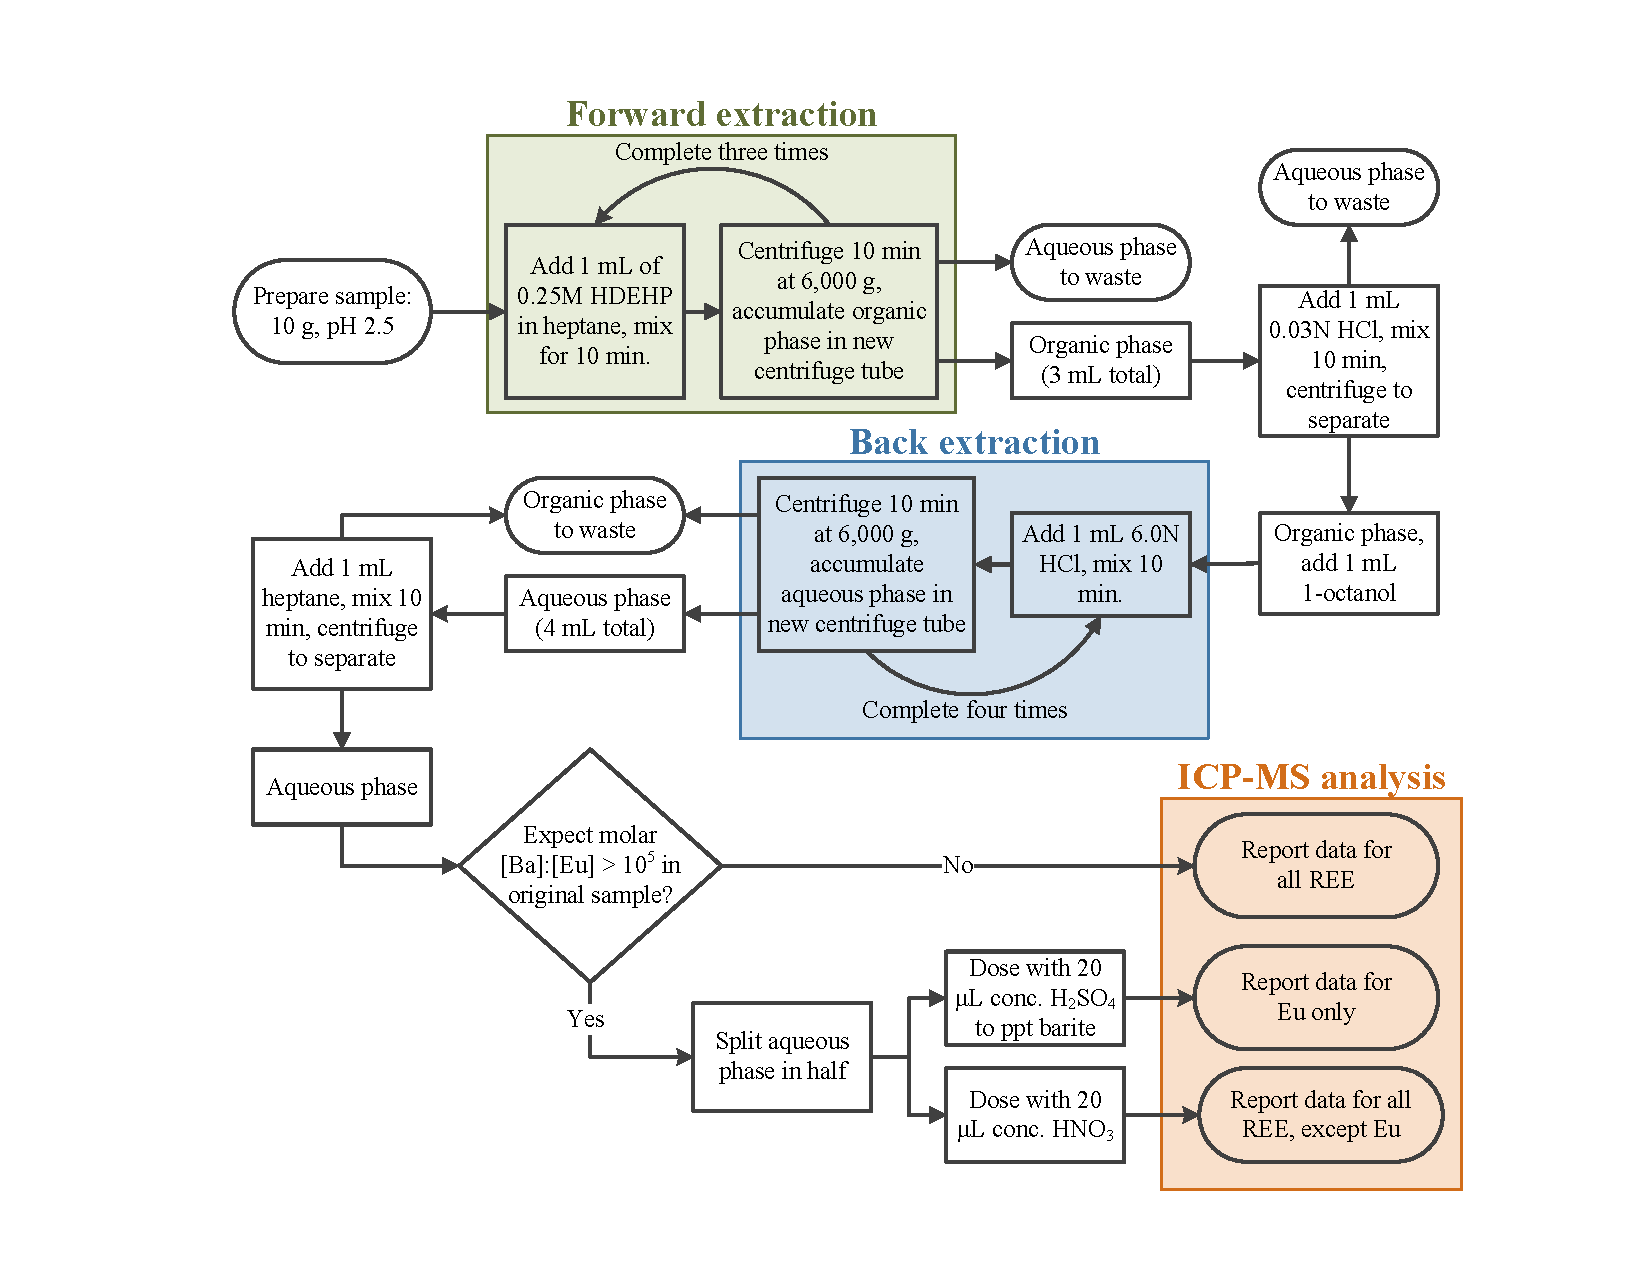
\includegraphics[width=0.8\textwidth]{Ch4_figures/LLE-flowsheet.pdf}
\caption{Liquid-liquid extraction method flowsheet for separation and concentration of REE from small volume, hypersaline brines. The decision node for the [Ba]:[Eu] molar ratio assumes a \ce{BaO+} formation rate on the order of 0.1\% in the ICP-MS.}\label{fig:flowsheet}
\end{center}
\end{sidewaysfigure}

Synthetic brine solutions were adjusted to pH 2.5 in 50 mL PP centrifuge tubes with \ce{HNO3} and subsequently split into 10 g aliquots in 15 mL PP centrifuge tubes for replicate experiments.
For each aliquot or sample, the process for REE extraction and recovery is as follows.
One (1) mL of 0.25 M HDEHP in heptane was added to the aqueous solution.
HDEHP was used as complexing agent for REE.
The phases were emulsified and mixed end over end for 10 minutes.
The phases were separated by centrifugation at 6,000$\times$g for 10 minutes and the light organic phase was removed from the centrifuge tube via pipette and accumulated in a new centrifuge tube, retaining the aqueous phase in the original tube.
This process, whereby the REE are complexed with HDEHP and partitioned into the heptane (termed forward extraction), was completed a total of three times.
Following the third forward extraction, the aqueous phase was discarded.

To remove any matrix (Na, Fe, etc.) and interfering species (i.e. Ba) that partitioned during forward extraction, the accumulated organic phase (3 mL total) was rinsed with 1 mL of pH 1.5 HCl.
This mixture was emulsified and separated by the same methods as the forward extraction.
Once separated, the dense aqueous phase was removed via pipette and discarded.

A concentrated acid solution was used to dissociate the REE-HDEHP complexes and return the REE to an aqueous phase (termed back extraction).
To decrease the REE-HDEHP complexation strength and encourage complete recovery,29
1 mL of 1-octanol was added to the organic phase.
Back extraction was achieved with four, sequential steps of stripping with 1 mL of 6.0 N HCl (collecting the eluted REE in a total of 4 mL acid).
As with the forward extraction, the sample was emulsified and mixed end over end for 10 minutes and then separated via centrifugation at 6,000$\times$g for 10 minutes.
After centrifugation the aqueous phase was removed via pipette and accumulated in a separate centrifuge tube, retaining the organic phase in the original tube.
Following the four back-extractions, the organic phase was discarded.

The collected acid volume (4 mL) was then rinsed with 1 mL of heptane to remove any dissolved organics from the aqueous phase.
Phase mixing and separation were accomplished in the same manner as all other steps.
Following centrifugation, the dense aqueous phase was removed and analyzed.

Preliminary experiments (see Supporting Information, SI, SI1. ``Barium removal''; Figure S1) indicated that, while Ba was successfully removed in the course of the LLE ($>99.9\%$ average reduction) and the HEHe-mode collision cell in the ICP-MS was successfully limiting \ce{^{135}Ba^{16}O+} interferences with \ce{^{151}Eu+} (\ce{^{135}Ba^{16}O+}:\ce{^{135}Ba+} $\sim0.2\%$ on average), initial Ba concentrations were so high that ppb level, background Eu concentrations were observed (SI2. ``Background REE concentration'', Figure S2).
Thus, in order to determine Eu accurately in these synthetic brines an additional step was tested, where an aliquot of the final, collected acid volume was dosed with 20 \si{\uL} concentrated sulfuric acid (\ce{H2SO4}) to precipitate any remaining barium as barite (\ce{BaSO4}).
Efficiency of Ba removal after \ce{H2SO4} addition is compared in Figure S2B and S2D.
It should be noted that this step was unnecessary for samples without Ba.

The methodology of Jenner et al.40 as modified by McGinnis et al.41 was employed to correct for matrix effects, isobaric interferences, and instrument drift during ICP-MS analysis.
Details of this methodology are provided in the SI3. ``Internal-external standardization for analytical corrections''.
Typical analytical uncertainty was between 3 and 5\%.
Because of high backgrounds of Gd in our laboratory and high Ba in the experiments, oxide corrections for \ce{^{137}Ba^{16}O+} interference on \ce{^{151}Eu+} and \ce{^{157}Gd^{16}O+} on \ce{^{173}Yb+} were applied as in Aries et al.42 after ICP-MS analysis.

\section{Materials and methods}\label{sec:MnM}

%\bibliographystyle{unsrtnat}
%\bibliography{Ch4_bib}
